\subsection{A escrita científica}
A necessidade da escrita científica é constante. Na universidade, ela é tida como o principal meio de troca de informações %entre as diferentes partes envolvidas 
no processo de difusão do conhecimento. Autores a utilizam em seus livros, pesquisadores divulgam suas descobertas através da publicação em revistas científicas, professores verificam o desempenho de seus alunos em avaliações escritas e os próprios acadêmicos a utilizam durante seus estudos. Na indústria, a escrita é valorizada na forma de relatórios técnicos, documentação de software e especificação de produtos.

Devido à sua importância, é natural que existam certas diretivas para se produzir um texto de forma correta e aqueles que não estão habituados a estas regras muitas vezes encontram dificuldades. Um problema frequente é o da apresentação visual dos documentos. No ambiente acadêmico, o interesse está no conteúdo de um trabalho e não em sua estética. Os artigos devem ser formatados seguindo uma norma padrão, geralmente definida pela instituição ou evento/revista no qual o trabalho está sendo divulgado. 

\subsection{Normas para escrita de trabalhos científicos}
A normas são definidas não de maneira aleatória, mas levando em consideração vários fatores como legibilidade do texto, tamanho do documento, local de publicação, presença de fórmulas matemáticas ou imagens, etc. Alguns dos detalhes presentes nas normas para escrita de artigos e trabalhos acadêmicos são: requisitos com relação à fontes, à disposição de parágrafos e seções, exibição de fórmulas e figuras, formatação de sumário e bibliografia.

Como estes detalhes são difíceis de serem capturados em palavras e regras, mostra-se abaixo um mesmo documento formatado de maneira a atender as regras de formatação do {\slshape Institute of Electrical and Electronics Engineers} (\textbf{IEEE}, acima) e da Sociedade Brasileira de Computação (\textbf{SBC}, abaixo).

Observe na página seguinte as diferenças com relação aos elementos de formatação do texto:
\begin{itemize}
\item Margens.
\item Estilos e tamanhos de fonte.
\item Centralização.
\item Forma de apresentar o nome dos autores.
\item Numeração das seções.
\item Tabulação dos parágrafos.
\end{itemize}

% Como exemplo do formato utilizado no padrão de conferências do IEEE, a página \pageref{IEEE} mostra o estilo de formatação necessário para submissão. Este formato é muito requisitado nos congressos internacionais e até mesmo para alguns eventos da SBC.

% No entanto, alguns congressos da SBC utilizam também formato próprio. Esse formato pode ser analisado na página \pageref{SBC}

Além disso, outro detalhe importante é a seção de referências. Cada congresso dispõe de maneiras diferentes para apresentação e citação das mesmas. Após a comparação entre a formatação dos textos, mostra-se, na página \pageref{referencias} as diferenças entre as referências das normas.

Repare como a citação do IEEE, na parte superior, ainda utiliza o formato de duas colunas, possui citação numérica, cita mais do que um autor e mostra maiores informações sobre a publicação em si. A norma da SBC, no meio, se parece mais com o padrão da UTFPR por ambas terem base na ABNT. As citações são por nome do autor e ano da publicação, e com menos informações sobre a obra. Por fim, as normas da UTFPR ressaltam o congresso publicado em negrito, autor todo em maiúsculo e mais metadados.

{\clearpage
\label{cabecalhos}
\newgeometry{left=0cm,bottom=0cm,top=0cm,right=0cm}

\noindent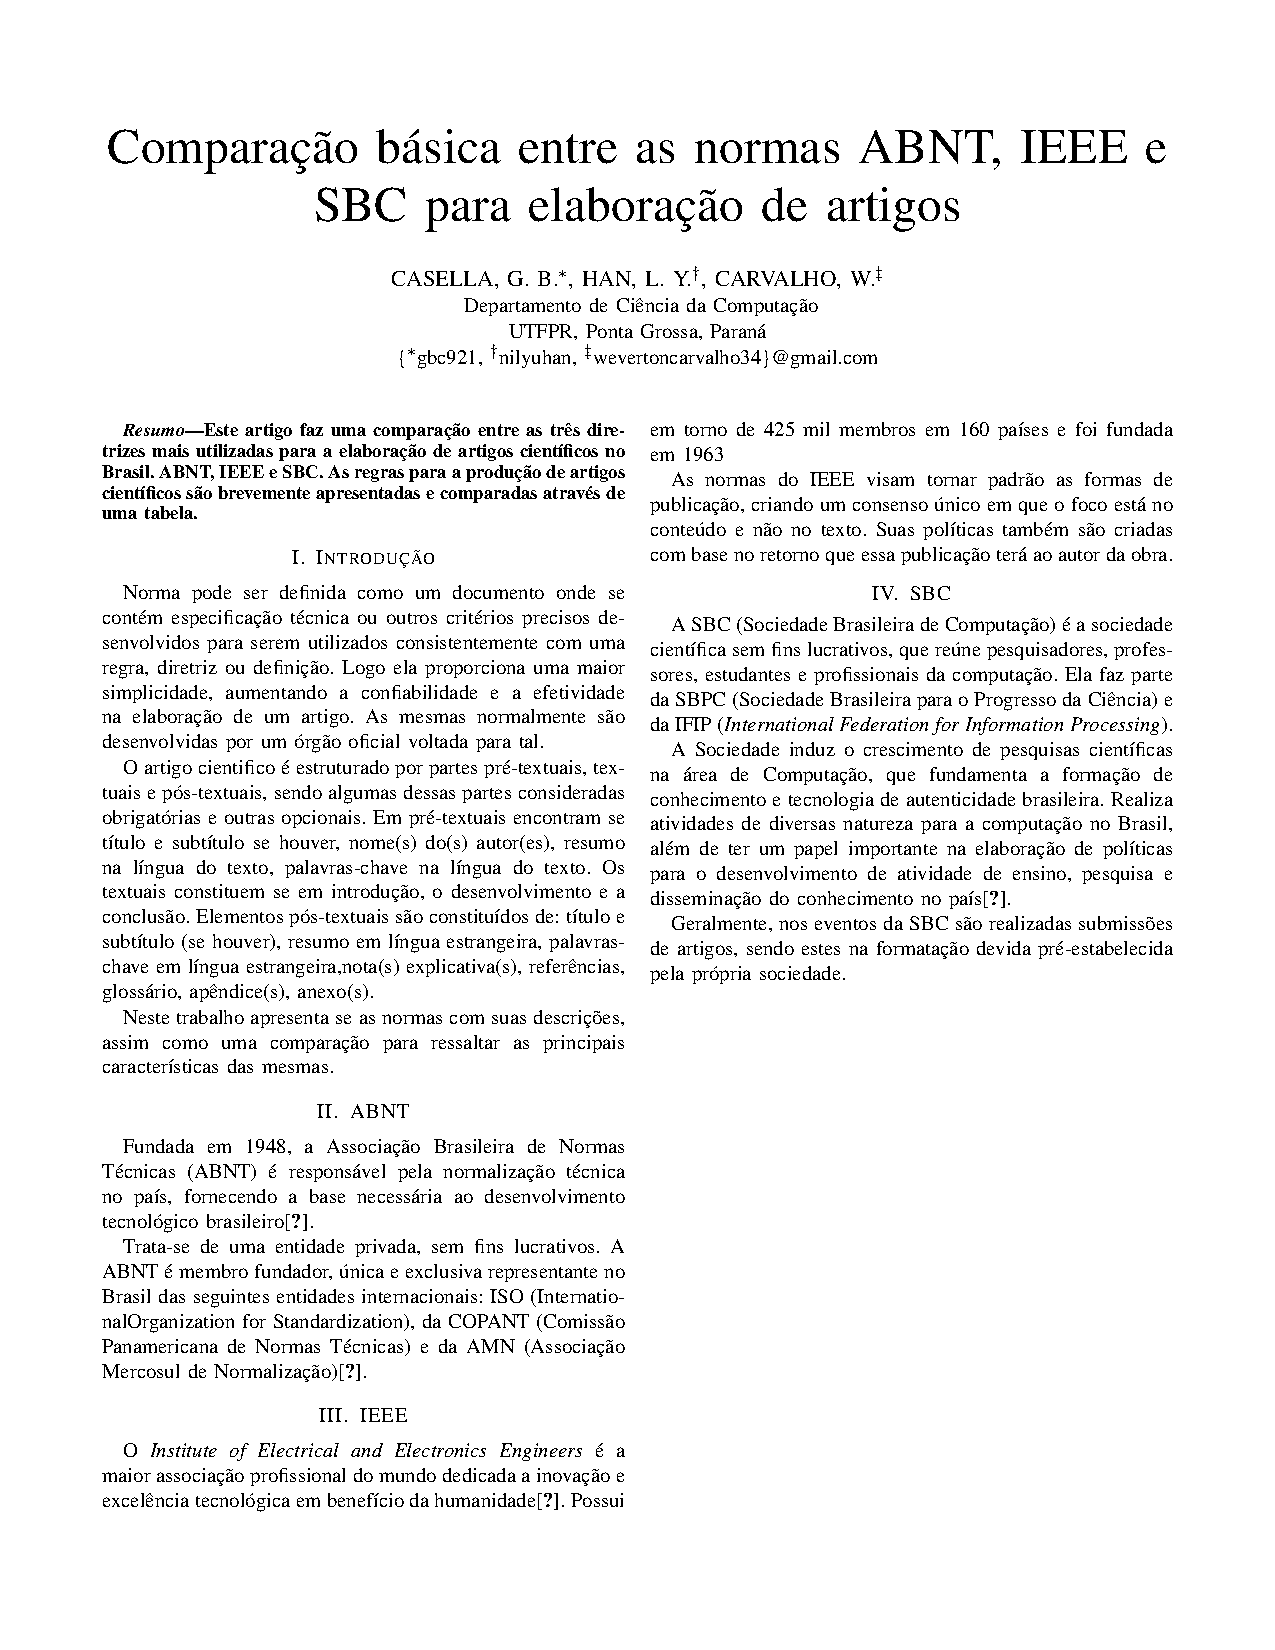
\includegraphics[trim=0 15cm 0 0,clip]{conteudo/intro_modelo_conferencias/intro_writing_ieee}

\hrule
%\noindent\hdashrule[0.5ex]{\textwidth}{2pt}{10pt}

\noindent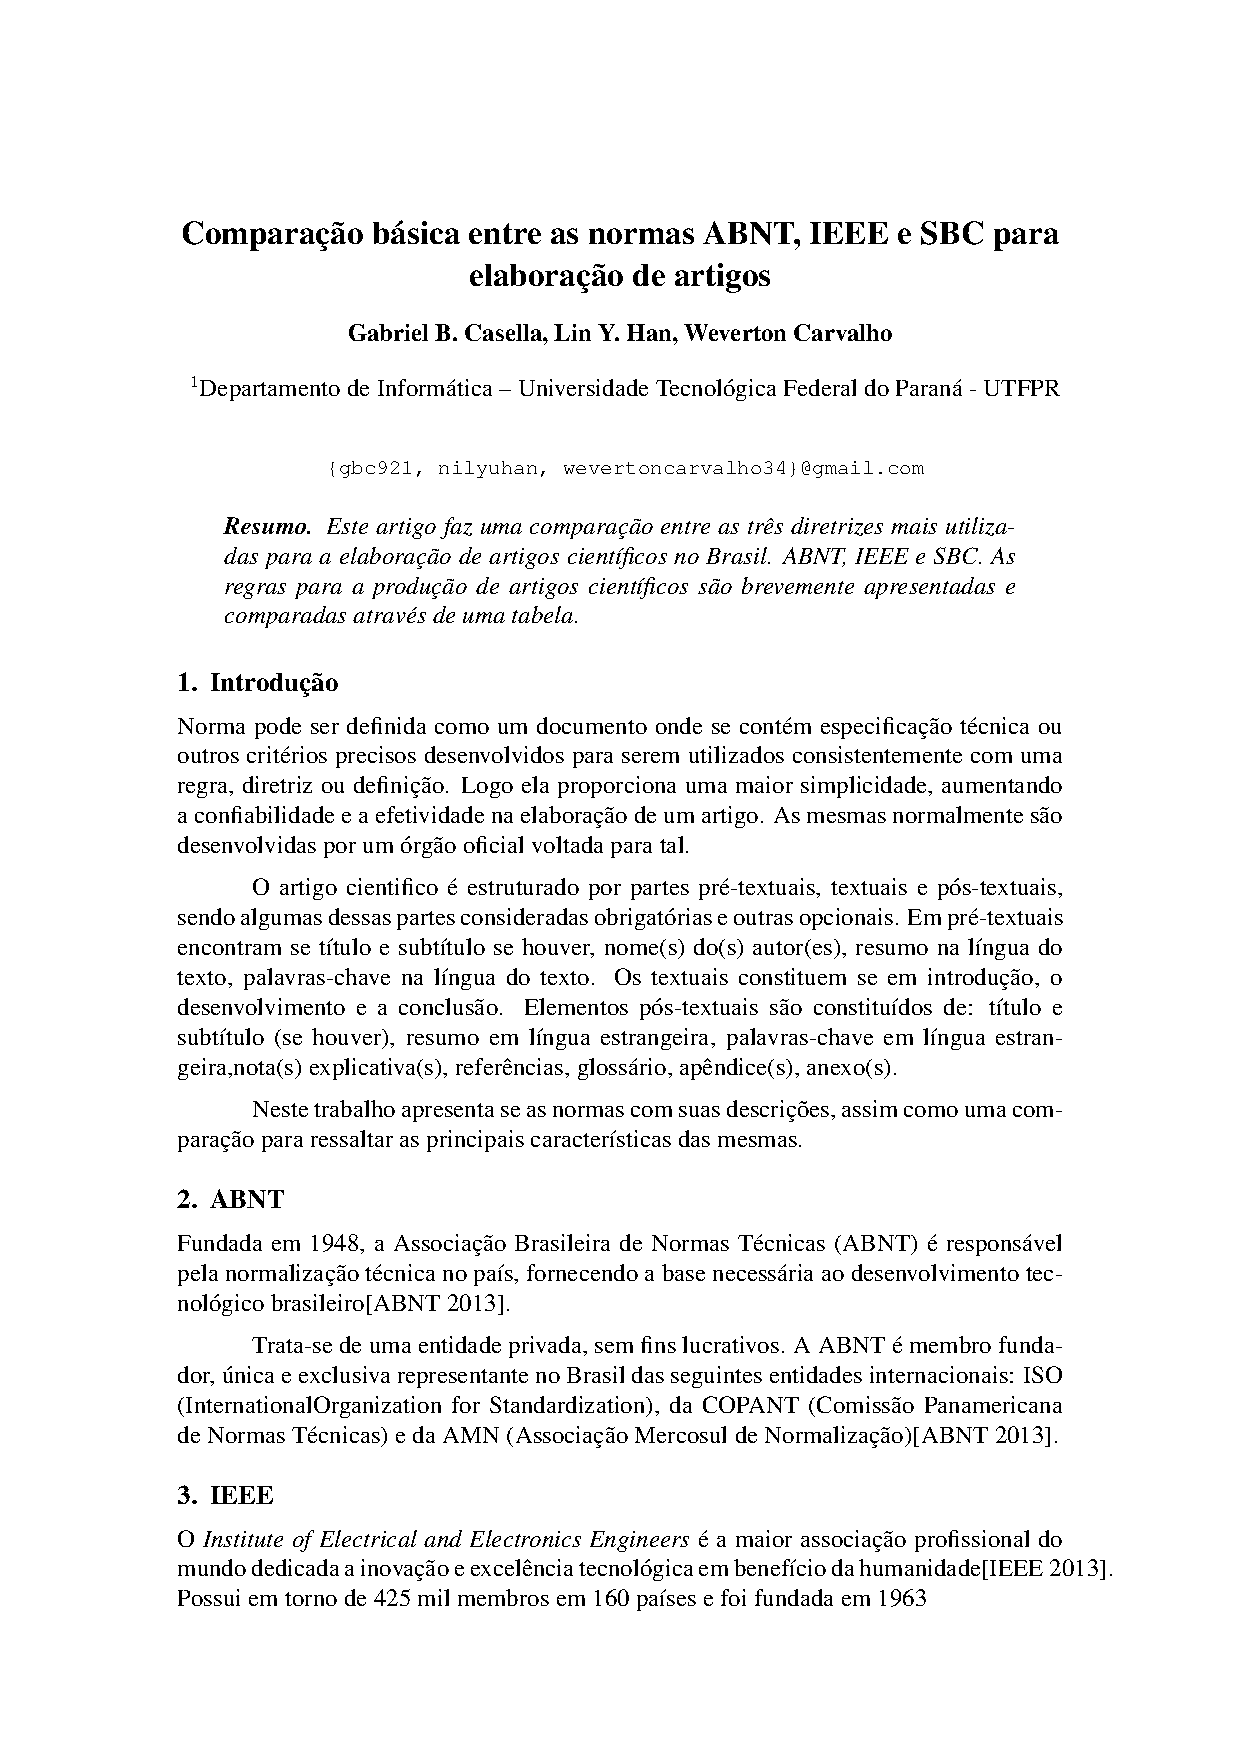
\includegraphics[trim=0 15cm 0 0,clip]{conteudo/intro_modelo_conferencias/intro_writing_sbc}

\clearpage}
\restoregeometry

 %Estes são apenas alguns dos detalhes que são exigidos e fica claro que a correta formatação de um documento é um processo que acaba ocupando uma grande parte do tempo dedicado à escrita do mesmo e 

{\clearpage
\label{referencias}
\newgeometry{left=0cm,bottom=0cm,top=0cm,right=0cm}

\noindent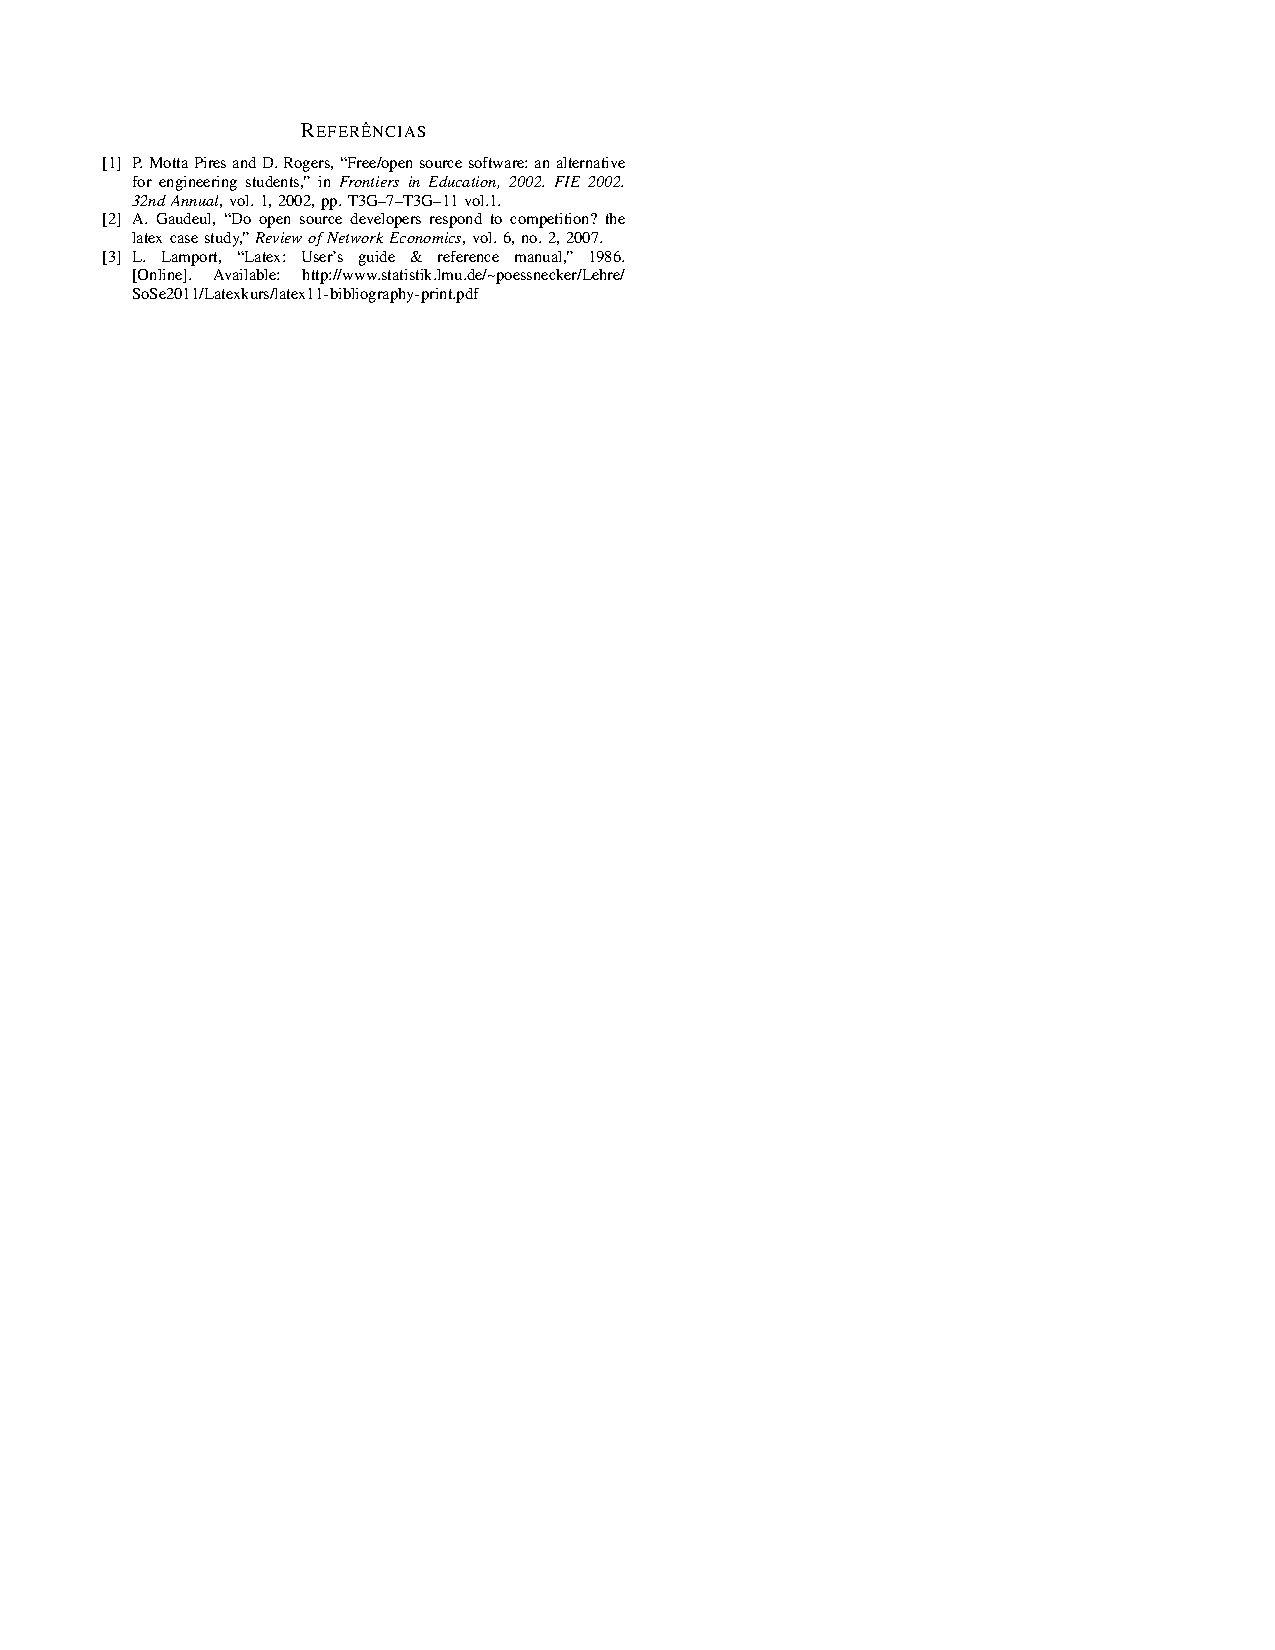
\includegraphics[trim=0 19cm 0 0,clip]{conteudo/intro_modelo_conferencias/references/ieee-refs}

\hrule

\noindent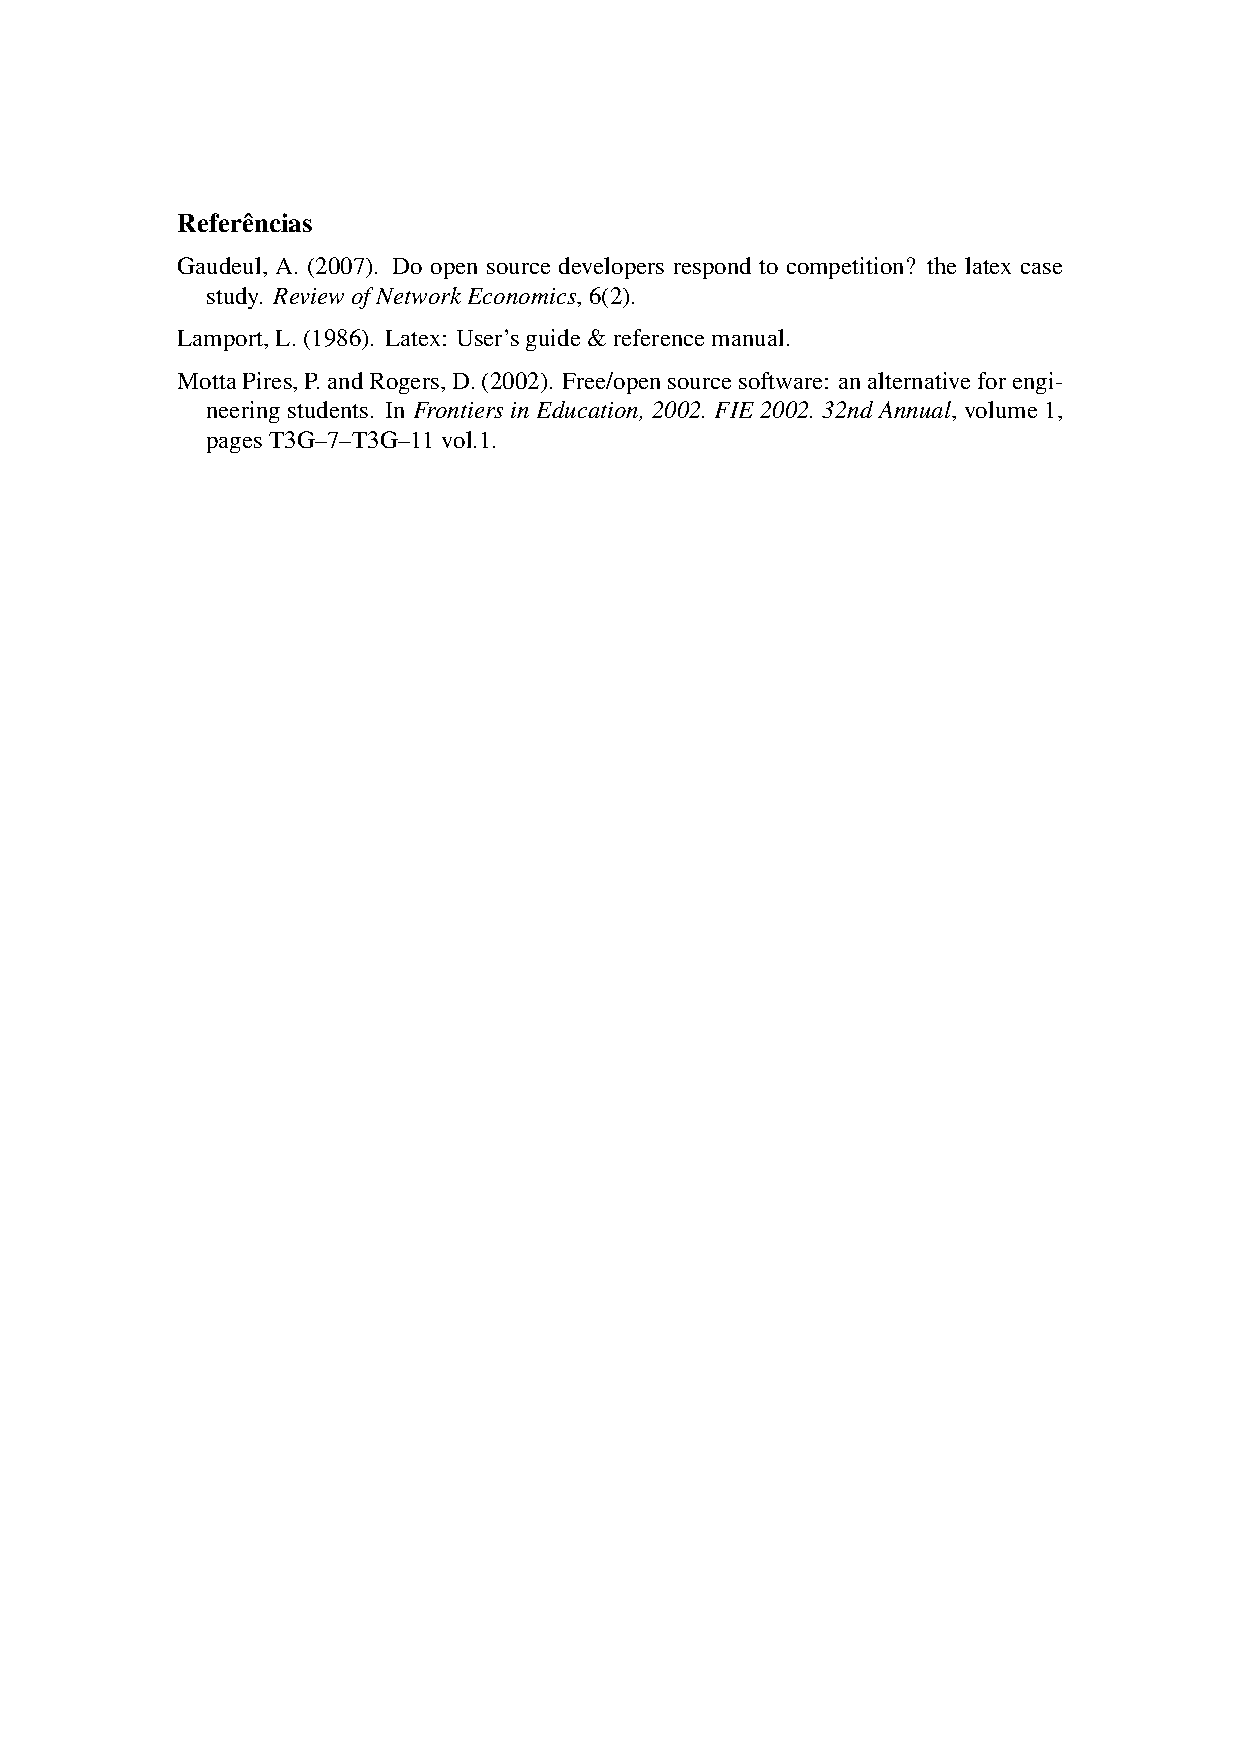
\includegraphics[trim=0 19cm 0 2cm,clip]{conteudo/intro_modelo_conferencias/references/sbc-refs}

\hrule
\noindent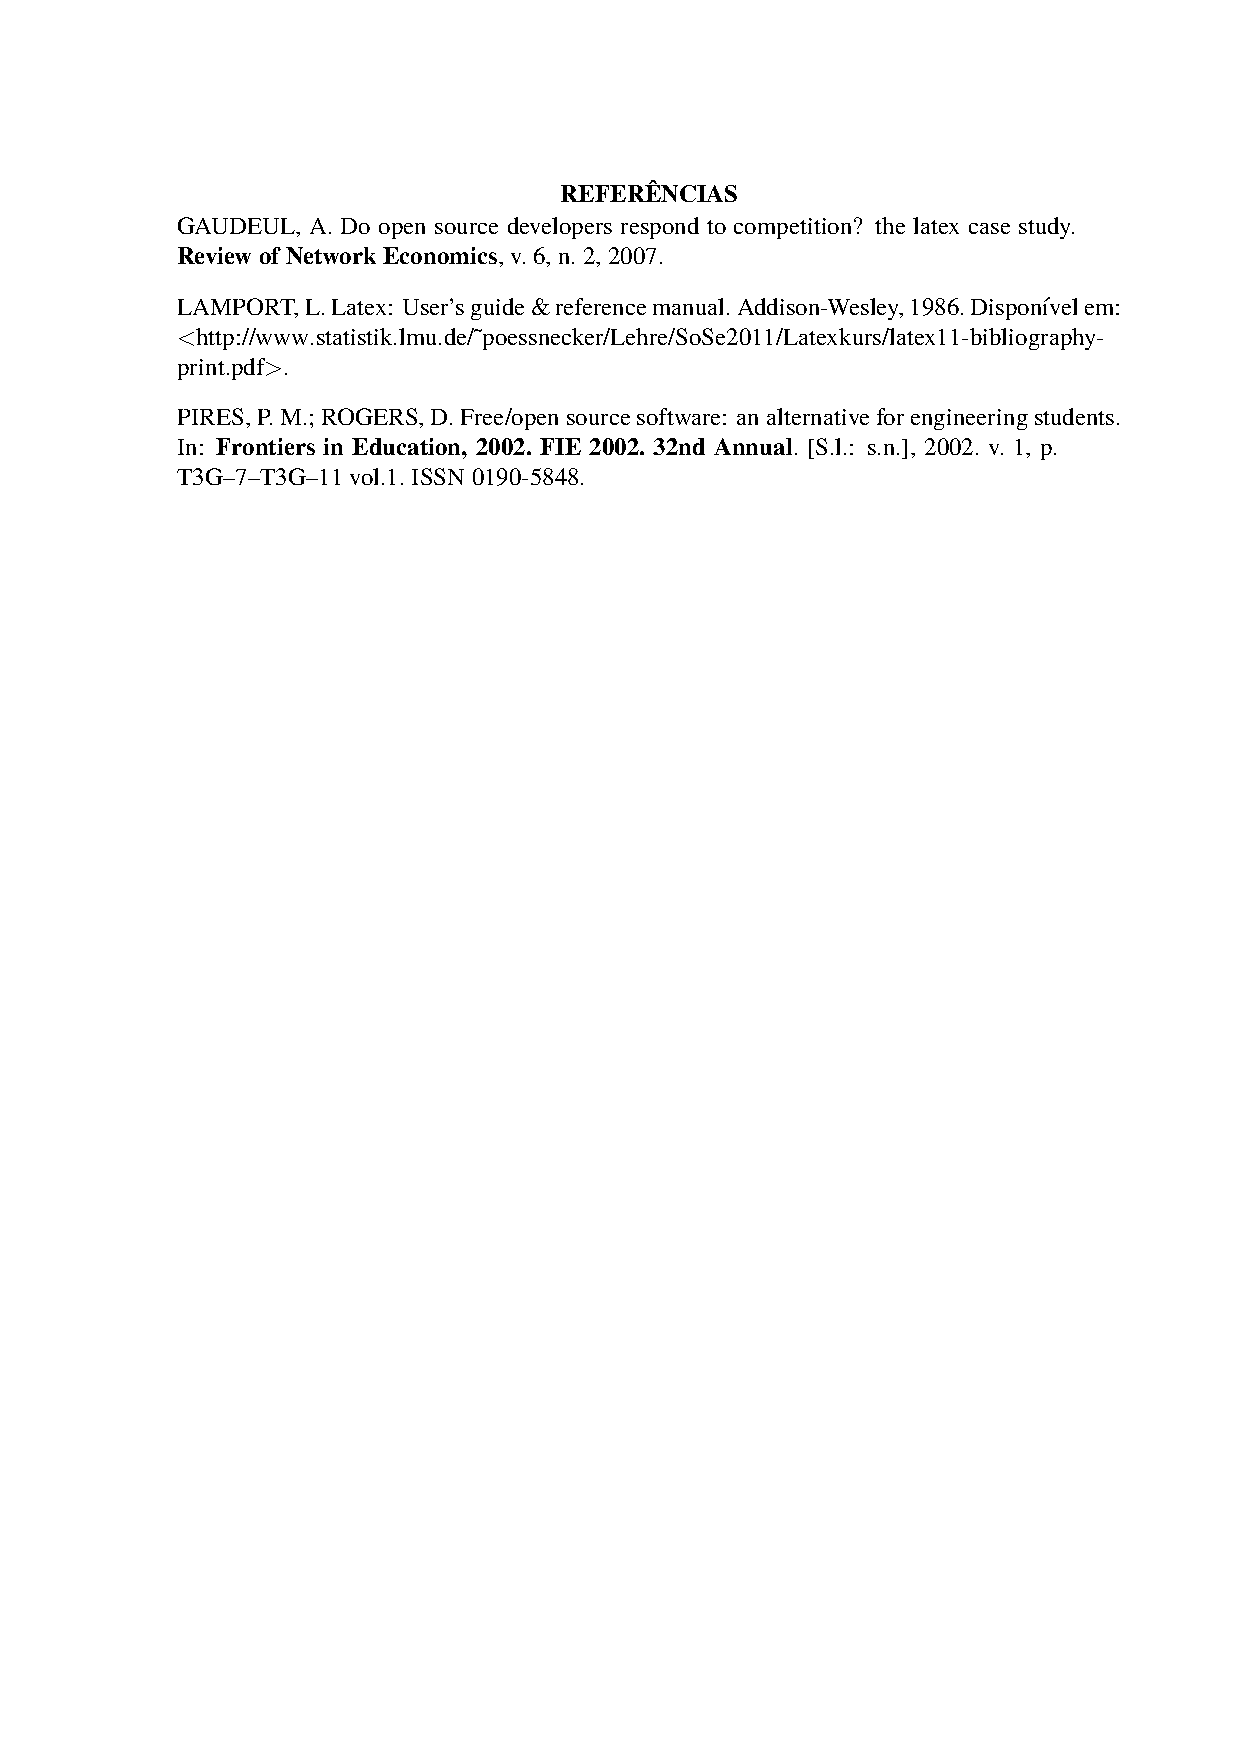
\includegraphics[trim=0 20cm 0 0cm,clip]{conteudo/intro_modelo_conferencias/references/utf-refs}

\clearpage}
\restoregeometry

Tendo em vista todos estes detalhes a serem levados em consideração bem como o fato de que os textos muitas vezes são escritos de maneira apressada devido a prazos curtos, como no caso de artigos ou relatórios de iniciação científica, fica claro que a utilização de ferramentas que automatizem e facilitem este processo de formatação serão sempre bem vindas. Uma destas ferramentas é o \LaTeX.

%Estes são apenas alguns dos detalhes que são exigidos e fica claro que a correta formatação de um documento é um processo que acaba ocupando uma grande parte do tempo dedicado à escrita do mesmo e a utilização de ferramentas que automatizem e facilitem este processo são sempre bem vindas. Uma destas ferramentas é o \LaTeX.


